
\chapter{引言}

\section{研究背景、目的和意义}
热液系统是洋中脊活动的重要组成部分,其热通量占全球总热通量的20-25\%,同时也在地表与地壳深部之间物质循环中扮演重要角色。
洋中脊热液系统也是研究生命起源以及新型生物群落的理想场所,在热液循环和生物化学作用下会形成有经济价值的金属矿床。
尤其近年来对超慢速扩张洋脊的调查发现,以岩浆集中供给为特征的超慢速扩张洋脊环境中的热液系统会形成大型多金属硫化物矿床。
中国大洋矿产资源研究与开发协会已于2011年11月,率先与国际海底管理局正式签署了《西南印度洋脊多金属硫化物勘探合同》。
本课题正是源于《多金属硫化物合同区资源勘探与评价》项目。
自2007年我国在西南印度洋脊发现第一个高温热液喷口以来,在西南印度洋合同区开展了一系列热液活动调查和地质取样,
在此区域海底获得了大量的地球物理、流体地球化学和岩石样品等资料,
但是对于海底一下的热液系统活动规律和热液流动的动力学特征尚不清楚,
而且通过深潜器和钻孔采集热液喷口数据和深部信息极度困难且昂贵。
因此,数值模拟方法是研究热液系统内部循环机制、动力学特征、物质和能量运移以及与矿物形成的关系的有力工具。
相比于快速和中速扩张洋脊,超慢速扩张洋脊的热液系统具有循环深度大、热源深度大、受断层控制作用强的特点。
目前国际上对快速、中速扩张洋脊的热液系统数值模拟研究较多,几乎没有对超慢速扩张洋脊环境下的超深(~16 km)的热液系统进行数值模拟研究。
因此,以建立超慢速扩张洋脊热液系统数值模型为研究内容,开展博士论文研究工作(以便于表述,如无特别说明,下文中所述的热液系统均指超慢速扩张洋脊热液系统)。


\section{研究现状和存在问题}
洋中脊热液系统数值模拟研究主要以国外研究机构(USGS, GEOMAR, ETH)为主,国内研究结构和学者对此领域研究较少。

\subsection{国内外研究现状和发展趋势}


耦合方案应该是求解这类问题的更好的选择,大的时间步长是的三维模拟更容易处理。但是问题在于如何推导出耦合方案既能保证稳定性又不失精度。

\subsection{存在问题和发展趋势}
对于洋中脊热液系统的数值模拟,


论文主要成果如下:

\begin{enumerate}
	\item 构建热液流体循环xxxx模拟方法
	\item 获得热液系统数值模拟程序,为后续研究打下了基础
	\item 发表两篇SCI 论文
\end{enumerate}



\section{模板使用方法}

\subsection{插入图片}
\begin{figure} [htbp] 
	\centering
	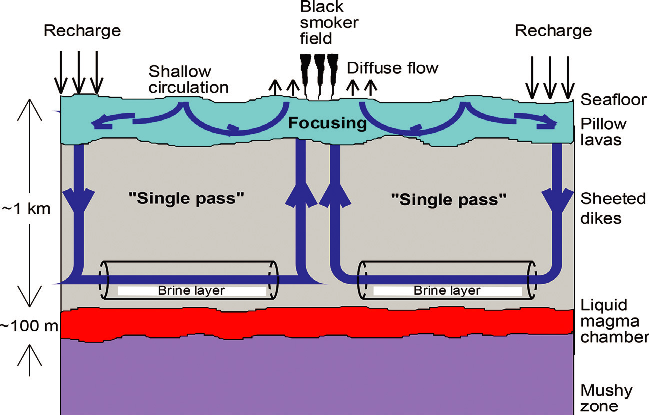
\includegraphics[width=\textwidth ]{SinglePassModel} 
	\caption[Single-pass model]{单通道模型} 
	\fnote{这是一段图注,乱按键盘:惊呆了撒娇来得及电路设计啊附近的骄傲而为的离开静安寺覅额黄飞鸿我积分对时间啊浪费我hi符合换个哈结尾覅哦啊见附件饿哦} 
	\label{fig:singlepassmodel} 
\end{figure} 

在这里引用此图,如图 \ref{fig:singlepassmodel} 所示。在论文末尾会自动生成插图索引。


\begin{figure} [htbp] 
	\centering
	
\includegraphics[width=0.5\textwidth ]{weixingongzhong} 
	\caption[Single-pass model]{Latex模板获取方法} 
	\fnote{扫码关注微信公众号并发消息\textcolor{red}{latex模板}即可获取模板文件} 
	\label{fig:template} 
\end{figure} 

在这里引用此图,如图 \ref{fig:singlepassmodel} 所示。在论文末尾会自动生成插图索引。

\subsection{表格}
表格与图类似,参见清华大学学位论文模板说明。

\subsection{公式}

行内公式,这个是行内公式 $E=MC^2$,下面是个带编号的独立公式:

\begin{equation}
	\frac{\partial T}{t} = \lambda \nabla T
	\label{eq:temperature}
\end{equation}

这里引用公式,公式\ref{eq:temperature}表示了温度的衰减。

\subsection{参考文献}
第一种引用方式:\cite{vehling2018implementation} 进行了相分离的数值模拟研究。
第二种引用方式:三维数值模拟目前仅限于单相流体\citep{coumou2008structure,coumou2006dynamics}。
这样的引用方式可能更易读一些,有可能地大要求以编号的形式显示,name只需要在main.tex里面把参考引用格式从{cugthesis-author-year}改为{cugthesis-numeric即可}